\chapter{Singular Value Decomposition}

Recall that a line through the origin in $\Re^n$ is 
$\set{r\cdot \vec{v}\suchthat r\in\Re}$. 
One of the defining properties of a linear map is that 
$h(r\cdot\vec{v})=r\cdot h(\vec{v})$.
So the action of $h$ on any 
line through the origin
is determined by the action
of $h$ on any nonzero vector in that line.

For instance consider the line~$y=2x$ in the plane.
\begin{equation*}
  \set{r\cdot\colvec{1 \\ 2}\suchthat r\in\Re}
\end{equation*}
If $\map{t}{\Re^2}{\Re^2}$ is represented by the matrix
\begin{equation*}
  \rep{t}{\stdbasis_2,\stdbasis_2}
  =
  \begin{mat}
    1 &2 \\
    3 &4
  \end{mat}
\end{equation*}
then here is the effect of $t$ on one vector in the line.
\begin{equation*}
  \colvec{1 \\ 2}\mapsunder{t}\colvec{7 \\ 10}
\end{equation*}
And here is the effect of $t$ on other members of the line.
\begin{equation*}
  \colvec{2 \\ 4}\mapsunder{t}\colvec{14 \\ 20}
  \qquad
  \colvec{-3 \\ -6}\mapsunder{t}\colvec{-21 \\ -30}
  \qquad
  \colvec{r \\ 2r}\mapsunder{t}\colvec{7r \\ 10r}
\end{equation*}
The map $t$'s action on the line is uniform.


\section{Unit circle}
The above means that one way to describe a transformation's action is to pick 
one nonzero element from each line through the origin and describe where
the transformation maps those elements.
An easy way to select one nonzero element from each line through the
origin is to take the upper half unit circle.
\begin{equation*}
  U=\set{\colvec{x \\ y}
         \suchthat 
         \text{$x=\cos(t)$, $y=\sin(t)$, $0\leq t<\pi$}}
  \qquad
  \vcenteredhbox{\includegraphics{sageoutput/plot_action10.png}}  
\end{equation*}
We produce the above 
graph by using a routine that draws the effect of an arbitrary 
matrix on the unit circle, and giving that routine the identity matrix. 
The colors will keep track the directionality in the set of
before and after pictures below.
\begin{sageoutput}
load "plot_action.sage"
p = plot_circle_action(1,0,0,1)  # identity matrix
p.set_axes_range(-1.5, 1.5, -0.5, 1.5) 
p.save("sageoutput/plot_action10.png")
\end{sageoutput}

Here 
is the transformation doubles the $x$~components of all vectors. 
\begin{sageoutput}[d,0,4;d,5,7]
load "plot_action.sage"
q = plot_circle_action(1,0,0,1) 
q.set_axes_range(-2, 2, -1, 2) 
q.save("sageoutput/plot_action11.png")
p = plot_circle_action(2,0,0,1) 
p.set_axes_range(-2, 2, -1, 2) 
p.save("sageoutput/plot_action11a.png")
\end{sageoutput}
\begin{equation*}
  \vcenteredhbox{\includegraphics{sageoutput/plot_action11.png}}
  \quad\mapsunder{\big (\begin{smallmatrix} 2 &0 \\ 0 &1 \end{smallmatrix}\big )}\quad
  \vcenteredhbox{\includegraphics{sageoutput/plot_action11a.png}}
\end{equation*}
And here is the
transformation that triples the $y$~components and multiplies 
$x$~components by $-1$. 

Note that it changes the orientation: the input circle moves 
counterclockwise from red to orange, then green, blue, indigo, and violet
but the output does the opposite. 
\begin{sageoutput}[d,0,4;d,5,7]
load "plot_action.sage"
q = plot_circle_action(1,0,0,1) 
q.set_axes_range(-2, 2, -4, 4) 
q.save("sageoutput/plot_action12.png")
p = plot_circle_action(-1,0,0,3) 
p.set_axes_range(-2, 2, -4, 4) 
p.save("sageoutput/plot_action12a.png")
\end{sageoutput}
\begin{equation*}
  \vcenteredhbox{\includegraphics{sageoutput/plot_action12.png}}
  \quad\mapsunder{\big (\begin{smallmatrix} -1 &0 \\ 0 &3 \end{smallmatrix}\big )}\quad
  \vcenteredhbox{\includegraphics{sageoutput/plot_action12a.png}}
\end{equation*}

Here is the first skew
transformation. 
\begin{sageoutput}[d,0,4;d,5,7]
load "plot_action.sage"
q = plot_circle_action(1,0,0,1) 
q.set_axes_range(-2, 2, -3, 3) 
q.save("sageoutput/plot_action13.png")
p = plot_circle_action(1,0,2,1) 
p.set_axes_range(-2, 2, -3, 3) 
p.save("sageoutput/plot_action13a.png")
\end{sageoutput}
\begin{equation*}
  \vcenteredhbox{\includegraphics{sageoutput/plot_action13.png}}
  \quad\mapsunder{\big (\begin{smallmatrix} 1 &0 \\ 2 &1 \end{smallmatrix}\big )}\quad
  \vcenteredhbox{\includegraphics{sageoutput/plot_action13a.png}}
\end{equation*}
\noindent Here is the second skew
transformation. 
\begin{sageoutput}[d,0,4;d,5,7]
load "plot_action.sage"
q = plot_circle_action(1,0,0,1) 
q.set_axes_range(-3, 3, -2, 2) 
q.save("sageoutput/plot_action14.png")
p = plot_circle_action(1,3,0,1) 
p.set_axes_range(-3, 3, -2, 2) 
p.save("sageoutput/plot_action14a.png")
\end{sageoutput}
\begin{equation*}
  \vcenteredhbox{\includegraphics{sageoutput/plot_action14.png}}
  \quad\mapsunder{\big (\begin{smallmatrix} 1 &3 \\ 0 &1 \end{smallmatrix}\big )}\quad
  \vcenteredhbox{\includegraphics{sageoutput/plot_action14a.png}}
\end{equation*}

And here is the generic map.
\begin{sageoutput}[d,0,4;d,5,7]
load "plot_action.sage"
q = plot_circle_action(1,0,0,1) 
q.set_axes_range(-2, 2, -4, 6) 
q.save("sageoutput/plot_action15.png")
p = plot_circle_action(1,2,3,4) 
p.set_axes_range(-2, 2, -4, 6) 
p.save("sageoutput/plot_action15a.png")
\end{sageoutput}
\begin{equation*}
  \vcenteredhbox{\includegraphics{sageoutput/plot_action15.png}}
  \quad\mapsunder{\big (\begin{smallmatrix} 1 &3 \\ 0 &1 \end{smallmatrix}\big )}\quad
  \vcenteredhbox{\includegraphics{sageoutput/plot_action15a.png}}
\end{equation*}



\section{SVD}
The above pictures show the unit circle mapping to ellipses.
Recall that in $\Re^2$ an ellipse has a \textit{major axis}, 
the longer one, and a 
\textit{minor axis}.\footnote{If the two axes have the same length 
then the ellipse is a circle.
If one axis has length zero then the ellipse is a line segment 
and if both have length zero then it is a point.}
Write $\sigma_1$ for the length of the semi-major axis, 
the distance from the center to the furthest-away point on the ellipse,
and write $\sigma_2$ for the length of the semi-minor axis.
\begin{sageoutput}[d,0,4]
plot.options['axes_pad'] = 0.05
plot.options['fontsize'] = 7
plot.options['dpi'] = 600
plot.options['aspect_ratio'] = 1
sigma_1=3
sigma_2=1
E = ellipse((0,0), sigma_1, sigma_2)
E.save("sageoutput/svd01.png", figsize=3.5)
\end{sageoutput}
\begin{center}
  \includegraphics{sageoutput/svd01.png}
\end{center}
The two axes are orthogonal.
In the above graph the major axis lies along the $x$-axis while the
minor axis lies along the $y$-axis.

Under any linear map $\map{t}{\Re^n}{\Re^m}$ the 
unit sphere maps to a hyperellipse.
This is a version of the \textit{Singular Value Decomposition} of
matrices:
for any linear map $\map{t}{\Re^m}{\Re^n}$ there are bases
$B=\sequence{\vec{\beta}_1,\ldots,\vec{\beta}_m}$ for the domain and
$D=\sequence{\vec{\delta}_1,\ldots,\vec{\delta}_n}$ for the codomain
such that $t(\vec{\beta}_i)=\sigma_i\vec{\delta}_i$, where the
\textit{singular values}
$\sigma_i$ are scalars.
The next section states that result more fully and sketches the proof
but first we illustrate the central idea by using the generic matrix.
Here is its action again, this time on a full circle.
\begin{sageoutput}[d,0,4;d,5,7]
load "plot_action.sage"
q = plot_circle_action(1,0,0,1,full_circle=True) 
q.set_axes_range(-2, 2, -5, 6) 
q.save("sageoutput/plot_action16.png")
p = plot_circle_action(1,2,3,4,full_circle=True) 
p.set_axes_range(-3, 3, -5, 6) 
p.save("sageoutput/plot_action16a.png")
\end{sageoutput}
\begin{equation*}
  \vcenteredhbox{\includegraphics{sageoutput/plot_action16.png}}
  \quad\mapsunder{\big (\begin{smallmatrix} 1 &2 \\ 3 &4 \end{smallmatrix}\big )}\quad
  \vcenteredhbox{\includegraphics{sageoutput/plot_action16a.png}}
  \tag{$*$}
\end{equation*}
\Sage{} will find the SVD of this example matrix.
\begin{sageoutput}
M = matrix(RDF, [[1, 2], [3, 4]])
U,Sigma,V = M.SVD()
U
Sigma
V
U*Sigma*(V.transpose())
\end{sageoutput}
\noindent 
The Singular Value Decomposition describes $M$ as the product of
three matrices, $U\Sigma\trans{V}$.
The basis vectors $\vec{\beta}_1$, $\vec{\beta}_2$, $\vec{\delta}_1$, 
and~$\vec{\delta}_2$ are the columns of $U$ and~$V$. 
The singular values are the diagonal entries of~$\Sigma$.
\Sage{} will plots the effect of the transformation
on the basis vectors for the domain so we can compare those with the
basis vectors for the codomain.
\begin{sageoutput}[d,0,2]
M = matrix(RDF, [[1, 2], [3, 4]])
U,Sigma,V = M.SVD()
beta_1 = vector(RR, [U[0][0], U[1][0]])
beta_2 = vector(RR, [U[0][1], U[1][1]])
delta_1 = vector(RR, [V[0][0], V[1][0]])
delta_2 = vector(RR, [V[0][1], V[1][1]])
plot.options['axes_pad'] = 0.05
plot.options['fontsize'] = 7
plot.options['dpi'] = 600
plot.options['aspect_ratio'] = 1
C = circle((0,0), 1)
P = C + plot(beta_1) + plot(beta_2)
P.save("sageoutput/svd02a.png", figsize=2, axes_pad=0.05)
image_color=Color(1,0.5,0.5)   # color for t(beta_1), t(beta_2)
Q = C + plot(beta_1*M, width=3, color=image_color) 
Q = Q + plot(delta_1,width=1.4,color='blue') 
Q = Q + plot(beta_2*M,width=3,color=image_color) 
Q = Q + plot(delta_2,width=1.4,color='blue')
Q.save("sageoutput/svd02b.png", figsize=4.467, axes_pad=0.05)
\end{sageoutput}
In the picture below, the domain's 
blue $\vec{\beta}$'s on the left map to the light red vectors on the
right.
Also on the right, in blue, are the $\vec{\delta}$'s.
The red $t(\vec{\beta}_1)$ does look to be about $5.5$ times $\vec{\delta}_1$,
and $t(\vec{\beta}_2)$ does look something like $0.4$ times~$\vec{\delta}_2$. 
\begin{equation*}
  % \setlength{\fboxsep}{0in} % used to set box heights by eye; surrounded each picture env with a fbox
  \setlength{\unitlength}{1in}
  \begin{picture}(1.35,1.35)
    \put(0,1.825){\includegraphics{sageoutput/svd02a.png}}
    \put(.3,1.9){\scriptsize $\vec{\beta}_1$}
    \put(0,2.7){\scriptsize $\vec{\beta}_2$}
  \end{picture}
  \quad
  \raisebox{2.65in}{$\mapsunder{\big (\begin{smallmatrix} 1 &2 \\ 3 &4 \end{smallmatrix}\big )}$}
  \qquad
  \begin{picture}(2.45,3.15)
    % \vcenteredhbox{\includegraphics{sageoutput/svd02b.png}}
    \put(0,0){\includegraphics{sageoutput/svd02b.png}}
    \put(1.25,2){\scriptsize $\vec{\delta}_1$}
    \put(2.3,2.1){\scriptsize $\vec{\delta}_2$}
  \end{picture}
  \tag*{\raisebox{2.5in}{($**$)}}
\end{equation*}
Note also that the two bases are \textit{orthonormal}\Dash the unit circles help
us see that the bases are comprised of unit vectors, and further,
the two members of each basis are orthogonal.

Compare this diagram to the one before it 
labelled ($*$), which shows the effect of the matrix
on the unit circle.
We used the whole circle in ($*$) to spotlight the ellipse, 
to make it easier to see that in ($**$)
the longest red vector is a
semi-major axis of that ellipse and the shortest red vector is a 
semi-minor axis.


\section{Proof sketch}

\textit{This argument, 
adapted from \cite{BlankKrikorianSpring89},
is a sketch because it uses results that a typical reader has only 
seen in a less general version and because it relies on material from the
book that is in an optional section.
In addition, we'll consider only the case of a nonsingular matrix and map;
it shows the main idea, which is the point of a sketch.}

Consider an~$\nbyn{n}$ matrix~$T$ that is nonsingular, and the
nonsingular transformation~$\map{t}{\Re^n}{\Re^n}$ that is represented by
$T$ with respect to the standard bases.

Recall the Extreme Value Theorem from Calculus~I: for a continuous
function~$f$, if $D\subset \Re$ is a closed and bounded set then
the image $f(D)$ is also a closed and bounded 
set (see \cite{wiki:ExtremeValueThm}).
A generalization of that result gives that because the unit sphere in $\Re^n$
is closed and bounded then its image under~$t$ is closed and bounded.
The image is in fact an ellipsoid, although we won't prove it,
so we will call it that. 

Because the ellipsoid is closed and bounded it has a point furthest from the
origin.
Let $\vec{w}$ be a vector extending from the origin to that furthest point.
Let $\vec{v}$ be the member of the unit sphere that maps to $\vec{w}$.
Let $P$ be the plane that touches the sphere only at the endpoint of $\vec{v}$.
Let $Q$ be the image of $P$ under~$t$.
Since $t$ is one-to-one, $Q$ touches the ellipsoid only at~$\vec{w}$.
\begin{center}
  \includegraphics{asy/ellipsoid1.pdf}
\end{center}

The tangent plane~$P$ has the property that 
the set of vectors whose bodies lie in~$P$
are the set of vectors perpendicular to $\vec{v}$.
That is, if in the picture above we slide $P$ along the vector~$\vec{v}$ to
the origin then we have the subspace of $\Re^n$ of vectors perpendicular
to~$\vec{v}$.
This subspace has dimension~$n-1$. 
We will argue below 
that if we similarly slide $Q$ to the origin then we have the
set of vectors perpendicular to~$\vec{w}$.
With that we will have an argument by induction: we start constructing the 
bases~$B$ and~$D$ by taking $\vec{\beta}_1$ to be~$\vec{v}$, taking
$\sigma_1$ to be the length $\norm{\vec{w}}$, and taking
$\vec{\delta}_1$ to be $\vec{w}/\norm{\vec{w}}$.

So consider~$Q$.
First observe that there is a unique plane that touches the ellipsoid
only at~$\vec{w}$ since if there were another $\hat{Q}$ then $t^{-1}(\hat{Q})$
would be a second plane that only touches the sphere at~$\vec{v}$, which is
impossible.
To see that $Q$ is perpendicular to~$\vec{w}$ consider a sphere
centered at the origin whose radius is $\norm{\vec{w}}$.
This sphere has a plane tangent at the endpoint of~$\vec{w}$, 
which is perpendicular
to $\vec{w}$.
Because $\vec{w}$ ends at a point on the ellipsoid furthest from the origin,
the ellipsoid is entirely contained in the sphere, so this plane touches
the ellipsoid only at~$\vec{w}$.
Therefore, from the second sentence of this paragraph, this plane is~$Q$. 
That ends the proof.



\section{Matrix factorization}

We can express those geometric ideas in an algebraic form
(for a proof see \cite{TrefethenBau97}).

The \textit{singular value decomposition} of an $\nbym{m}{n}$ matrix~$A$
is a factorization $A=U\Sigma \trans{V}$.
The $\nbym{m}{n}$ matrix $\Sigma$ is 
is all zeroes except for diagonal entries, the singular values, 
$\sigma_1\geq \sigma_2 \geq \cdots \geq \sigma_r> 0$ where $r$ is the
rank of~$A$.
The $\nbyn{m}$ matrix~$U$ and the $\nbyn{n}$ matrix~$V$ are unitary, meaning
that their columns form an orthogonal basis of unit vectors, the left and 
right \textit{singular vectors} for~$A$, respectively. 
\begin{sageoutput}
M = matrix(RDF, [[0, 1, 2], [3, 4, 5]])
U,Sigma,V = M.SVD()
U
Sigma
V  
\end{sageoutput}
The number of singular values is the rank of the matrix.
Here \Sage{} gets a $\sigma_2$ that is not quite zero because of numerical 
issues. 
\begin{sageoutput}
M = matrix(RDF, [[0, 1, 2], [0, 2, 4]])
U,Sigma,V = M.SVD()
U
Sigma
V  
\end{sageoutput}

The product $U\Sigma\trans{V}$ simplifies.
To see how,
consider the case where all three matrices are $\nbyn{2}$.
Write $\vec{u}_1$, $\vec{u}_2$ for the columns of~$U$
and $\vec{v}_1$, $\vec{v_2}$ for the columns of~$V$,
so that the rows of $\trans{V}$ are $\trans{\vec{v}}_1$ and
$\trans{\vec{v}}_2$.
\begin{align*}
  U\Sigma \trans{V}
  &=
  \begin{mat}
    \vec{u}_1 &\vec{u}_2
  \end{mat}
  \begin{mat}
    \sigma_1 &0 \\
    0        &\sigma_2
  \end{mat}
  \begin{mat}
    \trans{\vec{v}}_1 \\[.75ex]
    \trans{\vec{v}}_2
  \end{mat}             \\[.5ex]
  &=
  \begin{mat}
    \vec{u}_1 &\vec{u}_2
  \end{mat}
  \begin{mat}
    \sigma_1 &0 \\
    0        &0
  \end{mat}
  \begin{mat}
    \trans{\vec{v}}_1 \\[.75ex]
    \trans{\vec{v}}_2
  \end{mat}             
  +
  \begin{mat}
    \vec{u}_1 &\vec{u}_2
  \end{mat}
  \begin{mat}
    0        &0 \\
    0        &\sigma_2
  \end{mat}
  \begin{mat}
    \trans{\vec{v}}_1 \\[.75ex]
    \trans{\vec{v}}_2
  \end{mat}             \\[.5ex]
  &=
  \sigma_1\cdot
  \begin{mat}
    \vec{u}_1 &\vec{u}_2
  \end{mat}
  \begin{mat}
    1 &0 \\
    0 &0
  \end{mat}
  \begin{mat}
    \trans{\vec{v}}_1 \\[.75ex]
    \trans{\vec{v}}_2
  \end{mat}             
  +
  \sigma_2\cdot 
  \begin{mat}
    \vec{u}_1 &\vec{u}_2
  \end{mat}
  \begin{mat}
    0        &0 \\
    0        &1
  \end{mat}
  \begin{mat}
    \trans{\vec{v}}_1 \\[.75ex]
    \trans{\vec{v}}_2
  \end{mat}
  \tag{$*{*}*$}
\end{align*}
We'll look at the first term.
Right multiplication by the $1,1$~unit matrix picks out the first column of
$U$ and left multiplication by the $1,1$~unit matrix picks out first row of
$V$ so those are the only parts that remain after the product.
In short, we get this.
\begin{equation*}
  \begin{mat}
    u_{1,1} &u_{1,2} \\
    u_{2,1} &u_{2,2}
  \end{mat}
  \begin{mat}
    1 &0 \\
    0 &0
  \end{mat}
  \begin{mat}
    v_{1,1} &v_{2,1} \\
    v_{1,2} &v_{2,2}
  \end{mat}
  =
  \begin{mat}
    u_{1,1}v_{1,1} &u_{1,1}v_{2,1} \\
    u_{2,1}v_{1,1} &u_{2,1}v_{2,1}
  \end{mat}
  =\vec{u}_1\trans{\vec{v}}_1
\end{equation*}
In this way equation~($*{*}*$) simplifies to
$U\Sigma \trans{V}=\sigma_1\cdot\vec{u}_1\trans{\vec{v}}_1
   +\sigma_2\cdot\vec{u}_2\trans{\vec{v}}_2$.
Cases other than~$\nbyn{2}$ simplify in the same way.



\section{Application: data compression}

We now can write any matrix as a sum
$M=\sigma_1\cdot\vec{u}_1\trans{\vec{v}}_1
   +\sigma_2\cdot\vec{u}_2\trans{\vec{v}}_2
   +\cdots$
where the vectors have unit size and the $\sigma_i$'s decrease in size.
So if we have data as a matrix then we could hope to compress it
with that formula by dropping terms with small $\sigma$'s.  

We will illustrate with image compression.
Meet Lenna.
This top third of a pinup is a standard test image
\cite{wiki:Lenna}.
\begin{center}
  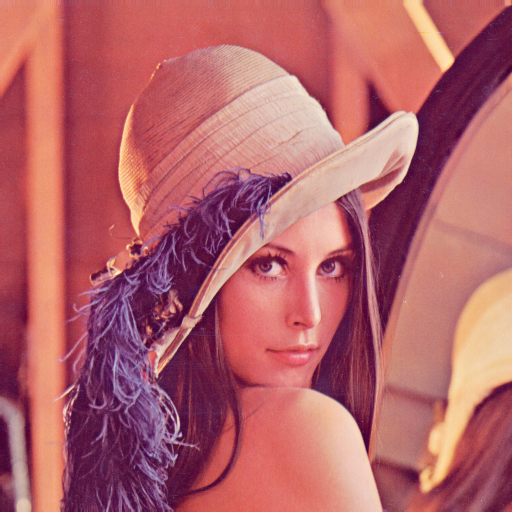
\includegraphics{Lenna.png} % from http://en.wikipedia.org/wiki/File:Lenna.png
\end{center}

We will use the Python Image Library for help in reading the figure, 
getting the color value at each pixel, etc.
This is a detour from Linear Algebra but in the image operations in 
the code below are clear to read.
\begin{sageoutput}
import Image
lena_img = Image.open("Lenna.png")
lena_img = lena_img.convert("RGB")
lena_img_rows, lena_img_cols = lena_img.size
\end{sageoutput}
We now have the image as a $\nbyn{512}$ array of pixels.
Each pixel is a triple 
$(\text{red}, \text{green},\text{blue})$ of integers that range from 
$0$ to~$255$.
Here we get the RGB triple for the pixel at location~$x=100$ and~$y=50$,
counting from the upper left of the picture and starting at $x=0$, 
$y=0$. 
\begin{sageoutput}[d,0,4]
import Image
lena_img = Image.open("Lenna.png")
lena_img = lena_img.convert("RGB")
lena_img_rows, lena_img_cols = lena_img.size
lena_img.getpixel((int(100), int(50)))
\end{sageoutput}
\noindent (The \inlinecode{int} function is a 
technicality: the Image module's \inlinecode{getpixel} function 
expects that the two numbers are Python integers, not a \Sage{}
integers.)

To use the \inlinecode{SVD} function we need \Sage{} matrices.
\Sage{} matrices are not mutable so we cannot build them up an entry at a time.
Instead we fetch the pixel color data into  
three Python arrays \inlinecode{rd}, \inlinecode{gr},
and \inlinecode{bl}.
Then we put that data as a whole 
into three \Sage{} matrices,\inlinecode{RD},
\inlinecode{GR} and~\inlinecode{BL}.
\begin{sageoutput}[d,0,4]
import Image
lena_img = Image.open("Lenna.png")
lena_img = lena_img.convert("RGB")
lena_img_rows, lena_img_cols = lena_img.size
rd, gr, bl = [], [], []
for row in range(lena_img_rows):
    rd.append([])
    gr.append([])
    bl.append([])
    for col in range(lena_img_cols):
        r, g, b = lena_img.getpixel((int(row),int(col)))
        rd[row].append(r)
        gr[row].append(g)
        bl[row].append(b)

RD, GR, BL = matrix(RDF, rd), matrix(RDF, gr), matrix(RDF, bl)
\end{sageoutput}

Now we take the Singular Value Decomposition of the three matrices.
Just out of curiosity, we have a peek at the eight largest singular
values in the red matrix, and the eight smallest.
\begin{sageoutput}[d,0,16]
import Image
lena_img = Image.open("Lenna.png")
lena_img = lena_img.convert("RGB")
lena_img_rows, lena_img_cols = lena_img.size
rd, gr, bl = [], [], []
for row in range(lena_img_rows):
    rd.append([])
    gr.append([])
    bl.append([])
    for col in range(lena_img_cols):
        r, g, b = lena_img.getpixel((int(row),int(col)))
        rd[row].append(r)
        gr[row].append(g)
        bl[row].append(b)

RD, GR, BL = matrix(RDF, rd), matrix(RDF, gr), matrix(RDF, bl)
U_RD,Sigma_RD,V_RD = RD.SVD()
U_GR,Sigma_GR,V_GR = GR.SVD()
U_BL,Sigma_BL,V_BL = BL.SVD()
for i in range(8):
    print "sigma_GR",i,"=",Sigma_GR[i][i]

for i in range(Sigma_GR.nrows()-8,Sigma_GR.nrows()):
    print "sigma_GR",i,"=",Sigma_GR[i][i]

\end{sageoutput}
The large singular values are much larger than the small singular values,
even setting aside those singular values that are zero except for numberical
issues.


Finally, for each matrix we will compute 
$\sigma_1\cdot\vec{u}_1\trans{\vec{v}}_1+\sigma_2\cdot\vec{u}_2\trans{\vec{v}}_2
   +\cdots$.
We have set the cutoff point at the fiftieth singular value, just because it
is close to ten percent of the total.

\begin{sageoutput}[d,0,19]
import Image
lena_img = Image.open("Lenna.png")
lena_img = lena_img.convert("RGB")
lena_img_rows, lena_img_cols = lena_img.size
rd, gr, bl = [], [], []
for row in range(lena_img_rows):
    rd.append([])
    gr.append([])
    bl.append([])
    for col in range(lena_img_cols):
        r, g, b = lena_img.getpixel((int(row),int(col)))
        rd[row].append(r)
        gr[row].append(g)
        bl[row].append(b)

RD, GR, BL = matrix(RDF, rd), matrix(RDF, gr), matrix(RDF, bl)
U_RD,Sigma_RD,V_RD = RD.SVD()
U_GR,Sigma_GR,V_GR = GR.SVD()
U_BL,Sigma_BL,V_BL = BL.SVD()
a=[]
for i in range(lena_img_rows): #
    a.append([])
    for j in range(lena_img_cols):
        a[i].append(0)

A_RD, A_GR, A_BL = matrix(RDF,a), matrix(RDF,a), matrix(RDF,a)
for i in range(50): #
    sigma_i = Sigma_RD[i][i]
    u_i = matrix(RDF, U_RD.column(i).transpose())
    v_i = matrix(RDF, V_RD.column(i))
    A_RD = copy(A_RD)+sigma_i*u_i*v_i
    sigma_i = Sigma_GR[i][i]
    u_i = matrix(RDF, U_GR.column(i).transpose())
    v_i = matrix(RDF, V_GR.column(i))
    A_GR = copy(A_GR)+sigma_i*u_i*v_i
    sigma_i = Sigma_BL[i][i]
    u_i = matrix(RDF, U_BL.column(i).transpose())
    v_i = matrix(RDF, V_BL.column(i))
    A_BL = copy(A_BL)+sigma_i*u_i*v_i
\end{sageoutput}
 




\section{Source of plot\_action.sage}
\lstinputlisting{plot_action.sage}

\endinput


TODO:
1) mention Sage matrices are not mutable in matrix introduction.
Is mutable discussed in Intro?